\section{Misura della caratteristica corrente-tensione di un resistore}
\subsection{Misura resistenza Voltmetro e Amperometro}
Per verificare che i lettori di grandezza di cui disponevamo fossero ben progettati, abbiamo proceduto analizzando due configurazoni differenti di circuiti.

Nella prima configurazione abbiamo disposto gli elementi circuitali come in figura:

\begin{figure}[h!]
    \centering
    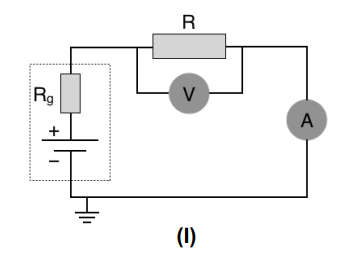
\includegraphics[scale=1]{Immagini/Conf1.PNG}
    \label{fig:my_label}
\end{figure}

Un lettore di tensione ideale dispone di una resistenza infinita; poichè nel caso reale non è possibile riporodurre questo fenomeno, si scelgono per i circuiti resistenze di ordini di grandezza molto minori di quelle dello strumento.
Abbiamo scelto la resistenza R, disposta in parallelo con quella del Voltmetro $R_{V}$, con un valore di $R=22M\Omega$. Questa scelta è stata motivata dal fatto che, per poter in seguito utilizzare resistenze con valori adatti, è stato necessario misurare quella del Voltmetro, confrontandola con un resistore che avesse un ordine di grandezza simile.
Riportiamo di seguito i dati raccolti, utilizzati per condurre un'interpolazione.

\begin{table}[H]
    \centering
    \begin{tabular}{cc}
    \toprule
    \Delta V (V)  & I (\mu A) \\
    \midrule
    0,507	&0,59\\
    1,012	&1,20\\
    1,527	&1,83\\
    2,032	&2,43\\
    2,544	&3,04\\
    3,051	&3,65\\
    3,56	&4,27\\
    \bottomrule
    \end{tabular}
    \label{tab:my_label}
\end{table}
 
\begin{figure}[H]
    \centering
    %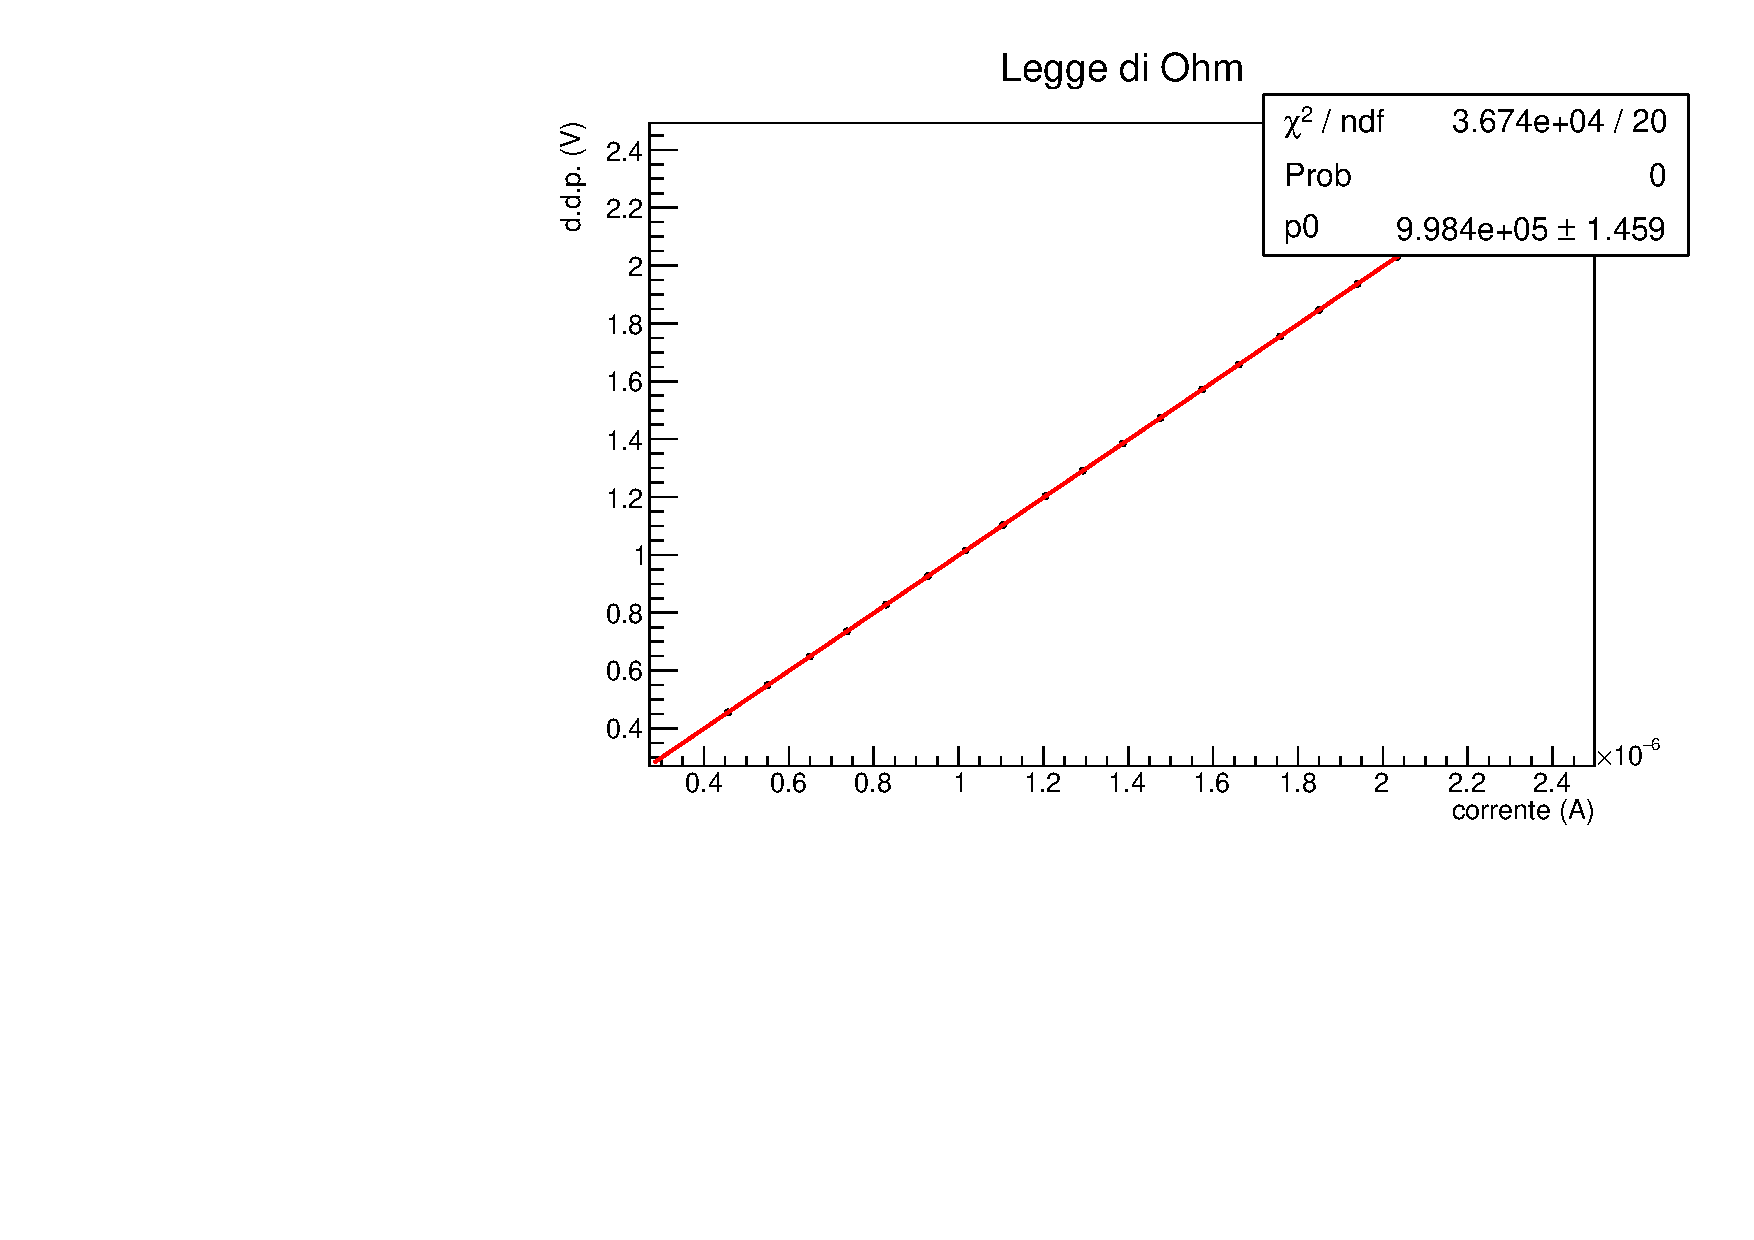
\includegraphics[scale=.5]{Immagini/Ohm configurazione 1.pdf}
    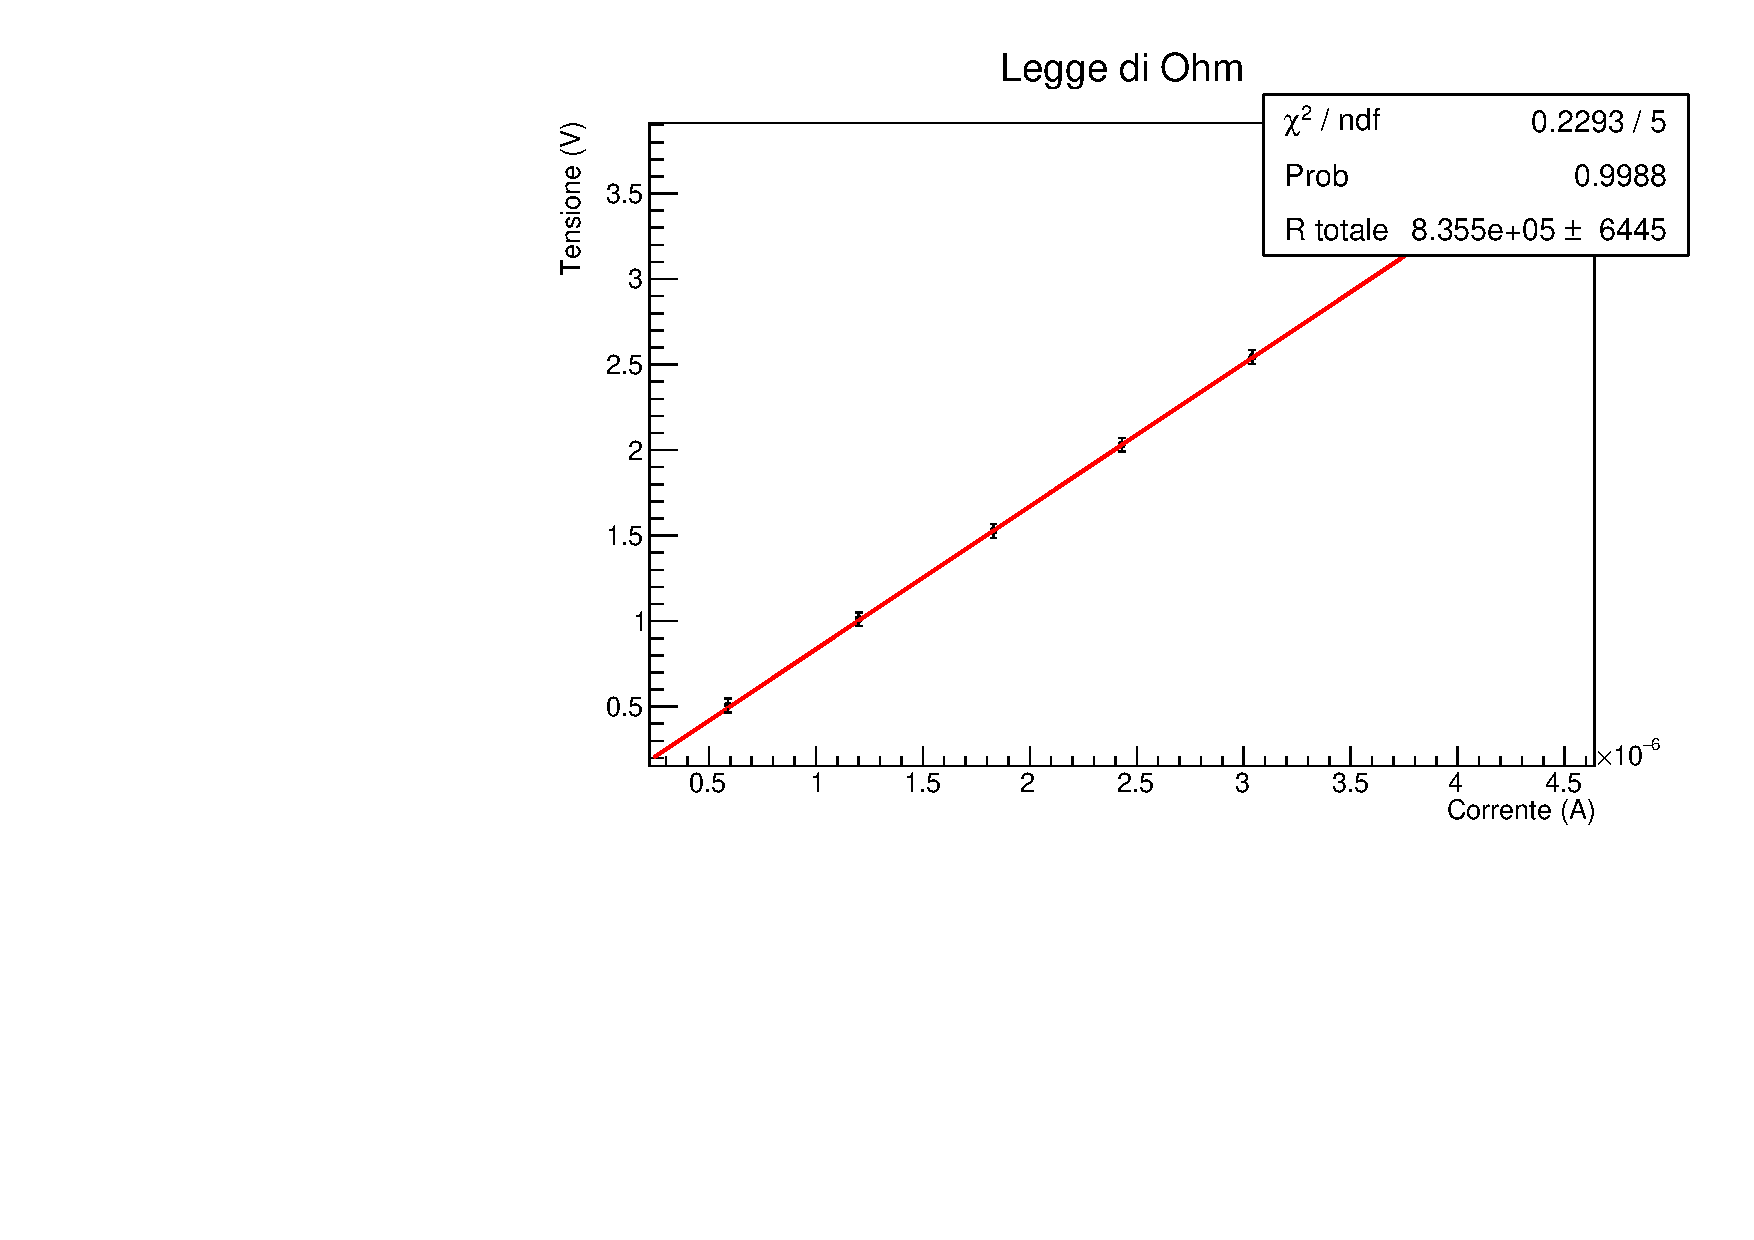
\includegraphics[scale=.5]{Immagini/fit1.pdf}
    \label{fig:my_label}
    \caption{Grafico configurazione Voltmetro}
\end{figure}

La resistenza del Voltmetro risulta essere di $1,05M\Omega$, essa dovrebbe, però, essere dell'ordine di grandezza di 10 $M\Omega$; discuteremo i motivi di questa incongruenza nelle conclusioni, ma crediamo possa essere attribuibile alla resistenza nota scelta.

Per il calcolo dell'errore abbiamo operato come segue:

$$
\sigma_{R_v}^2=\left[\sigma_{R_{equiv}}\left(\dfrac{\partial R_v}{\partial R_{equiv}}\right)\right]^2=\sigma^2_{R_{equiv}}\left(\dfrac{R_v^2}{(R_n -R_{tot}^2)}\right)^2=2,322 \Omega
\qquad \text{}
$$


Nella seconda configurazione abbiamo disposto gli elementi circuitali come in figura:

\begin{figure}[H]
    \centering
    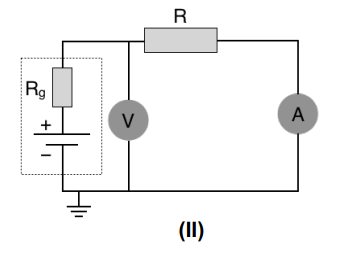
\includegraphics[scale=1]{Immagini/Conf2.PNG}
    \label{fig:my_label}
\end{figure}

Abbiamo scelto la resistenza R, disposta in serie con quella del Amperometro $R_{A}$, con un valore di $R=10\Omega$ per un motivo simile al precedente. A differenza del Voltmetro, l'Amperometro ideale ha una resistenza nulla, quindi, nella realtà, si scelgono resistori di ordini di grandezza molto maggiori dello strumento.
Anche in questo caso abbiamo deciso di condurre un'interpolazione per ricavare la resistenza equivalanente e, successivamente, quella dello strumento.

\begin{table}[H]
    \centering
    \begin{tabular}{cc}
    \toprule
    \Delta V (V)  & I (mA) \\
    \midrule
    1,016	&88,56\\
    1,515	&132,06\\
    2,026	&176,42\\
    2,533	&220,37\\
    3,044	&264,4\\
    3,549	&307,59\\
    4,061	&351,3\\
    \bottomrule
    \end{tabular}
    \label{tab:my_label}
\end{table}

\begin{figure}
    \centering
    %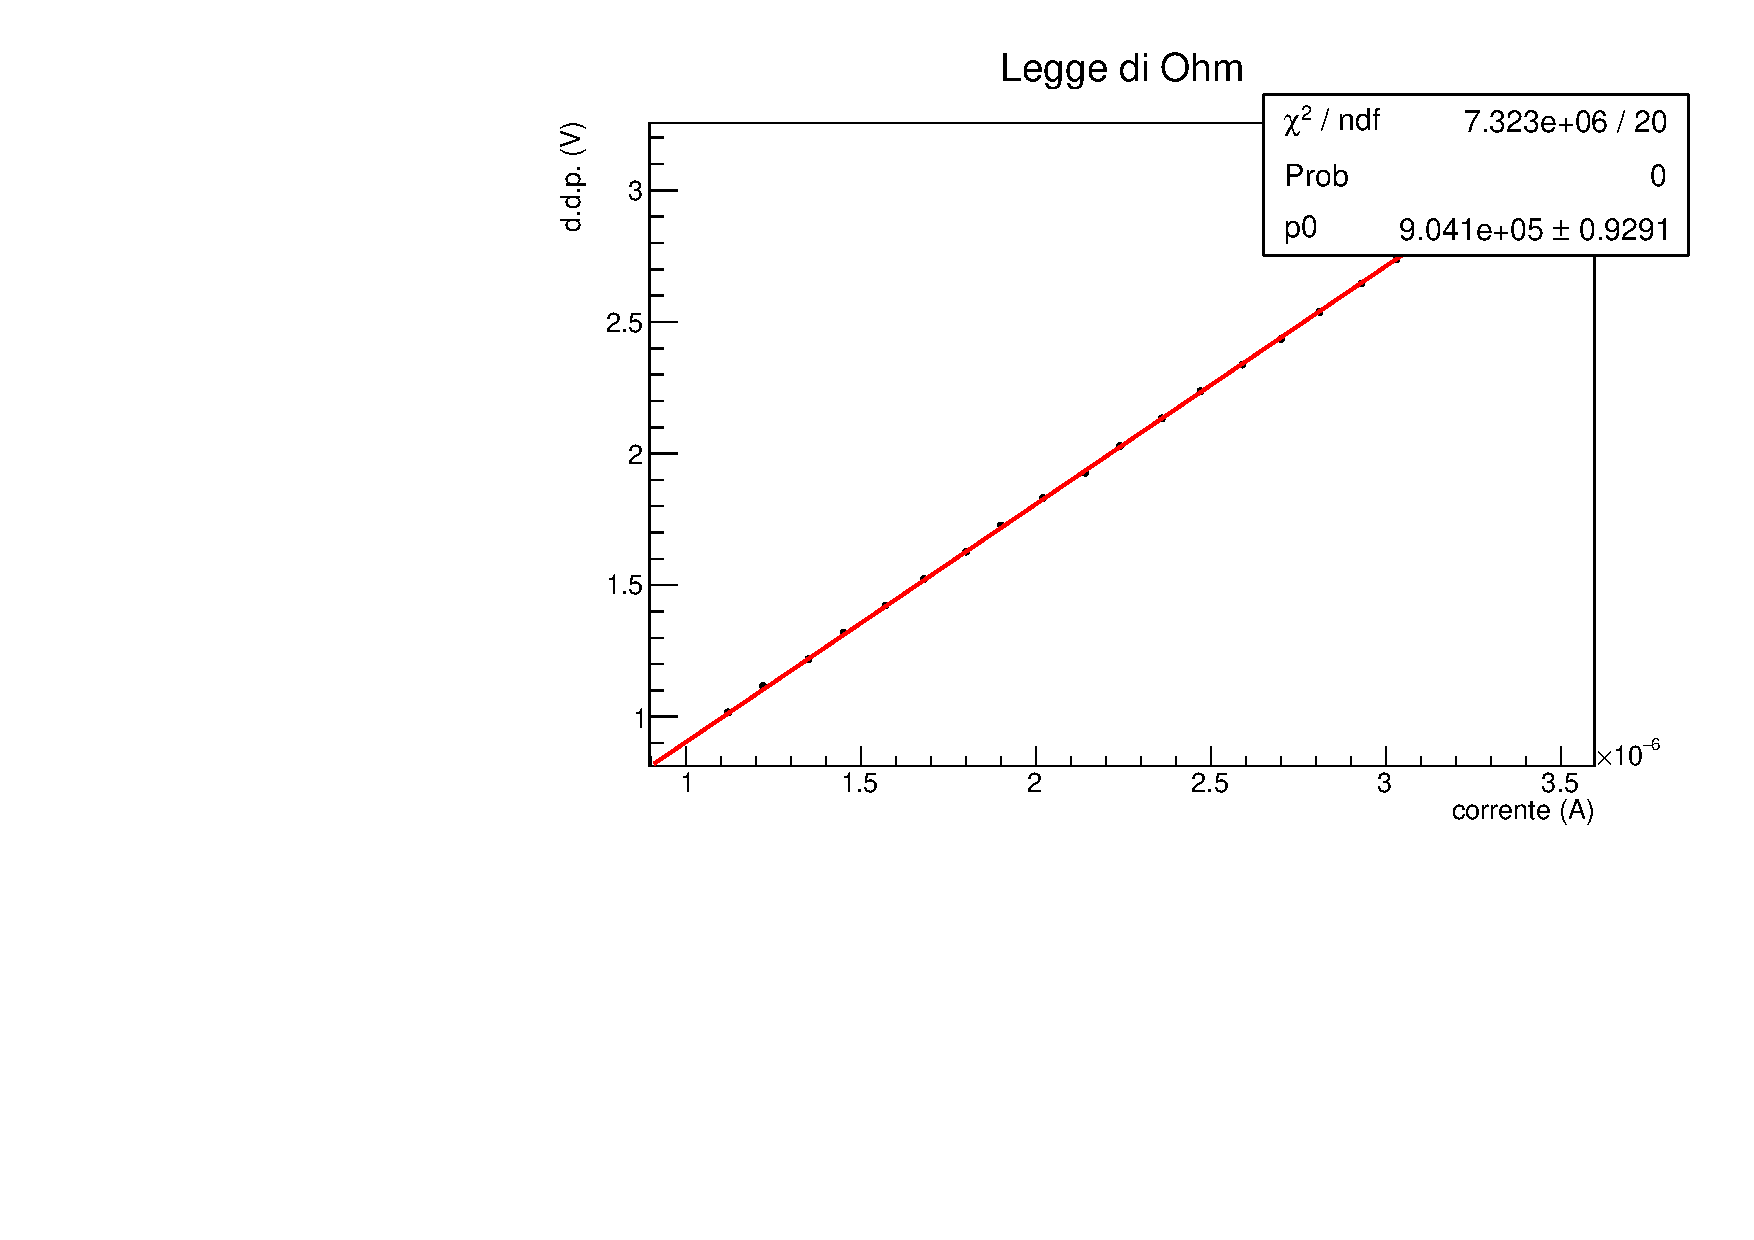
\includegraphics[scale=.5]{Immagini/Ohm configurazione 2.pdf}
    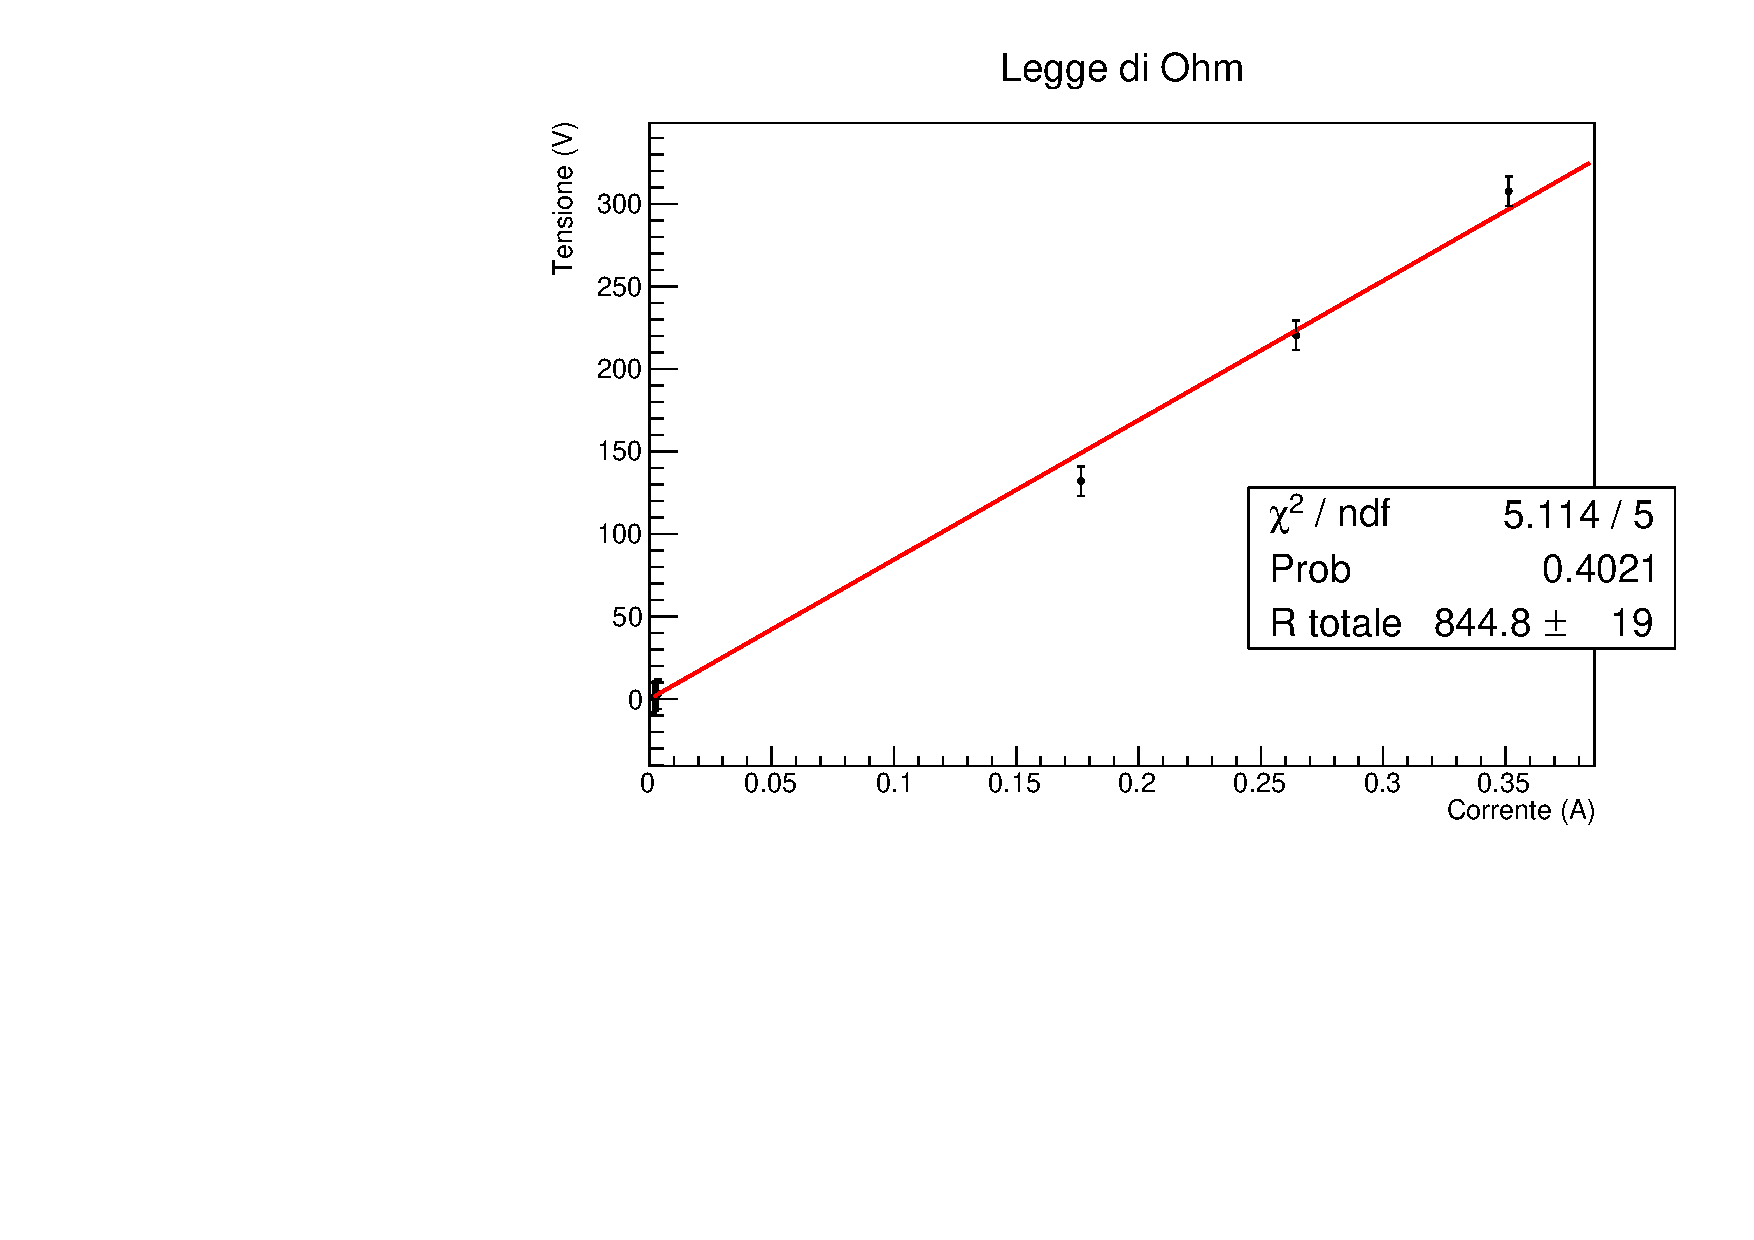
\includegraphics[scale=.5]{Immagini/fit2.pdf}
    \label{fig:my_label}
    \caption{Grafico configurazione Amperometro}
\end{figure}

Questo risultato risulta congruente con quello che ci aspettavamo.

\subsection{Verifica della legge di Ohm}
Successivamente, configurando correttamente entrambi i circuiti, abbiamo verificato la Legge di Ohm. Variando la misura della tensione di alimentazione del circuito, abbiamo misurato la differenza di potenziale ai capi del resistore e la corrente che lo attraversava.

\begin{table}[H]
\parbox{.45\linewidth}{
    \centering
    \begin{tabular}{cc|cc}
    \toprule
    \Delta V (V)  & I (mA) & \Delta V (V)  & I (mA) \\
    \midrule
    0,456	&0,45693 & 1,385	&1,3869\\
    0,55	&0,5497 & 1,474	&1,4761\\
    0,649	&0,6498 & 1,572	&1,5741\\
    0,736	&0,7372& 1,658	&1,6604\\
    0,828	&0,8293& 1,755	&1,7584\\
    0,927	&0,928& 1,847	&1,85\\
    1,015	&1,0166& 1,937	&1,9403\\
    1,103	&1,1048& 2,03	&2,0335\\
    1,203	&1,2048& 2,124	&2,128\\
    1,291	&1,293& 2,216	&2,2196\\
    2,308	&2,3126&&\\
    \bottomrule
    \end{tabular}
    \caption{Dati configurazione 1, R=1k\Omega}
    \label{tab:my_label}
}
\quad
\parbox{.45\linewidth}{
    \centering
    \begin{tabular}{cc|cc}
    \toprule
    \Delta V (V)  & I (\mu A) & \Delta V (V)  & I (\mu A) \\
    \midrule
    1,017	&1,12& 2,029	&2,24\\
    1,117	&1,22&2,134	&2,36\\
    1,219	&1,35& 2,237	&2,47\\
    1,319	&1,45&2,338	&2,59\\
    1,423	&1,57&2,436	&2,7\\
    1,524	&1,68&2,538	&2,81\\
    1,627	&1,8&2,646	&2,93\\
    1,727	&1,9&2,738	&3,03\\
    1,831	&2,02&2,85	&3,16\\
    1,927	&2,14&2,948	&3,27\\
    3,053	&3,37 &&\\
    \bottomrule
    \end{tabular}
    \caption{Dati configurazione 2, R=0,91M\Omega}
    \label{tab:my_label}
    }
\end{table}

\begin{figure}[H]
    \centering
    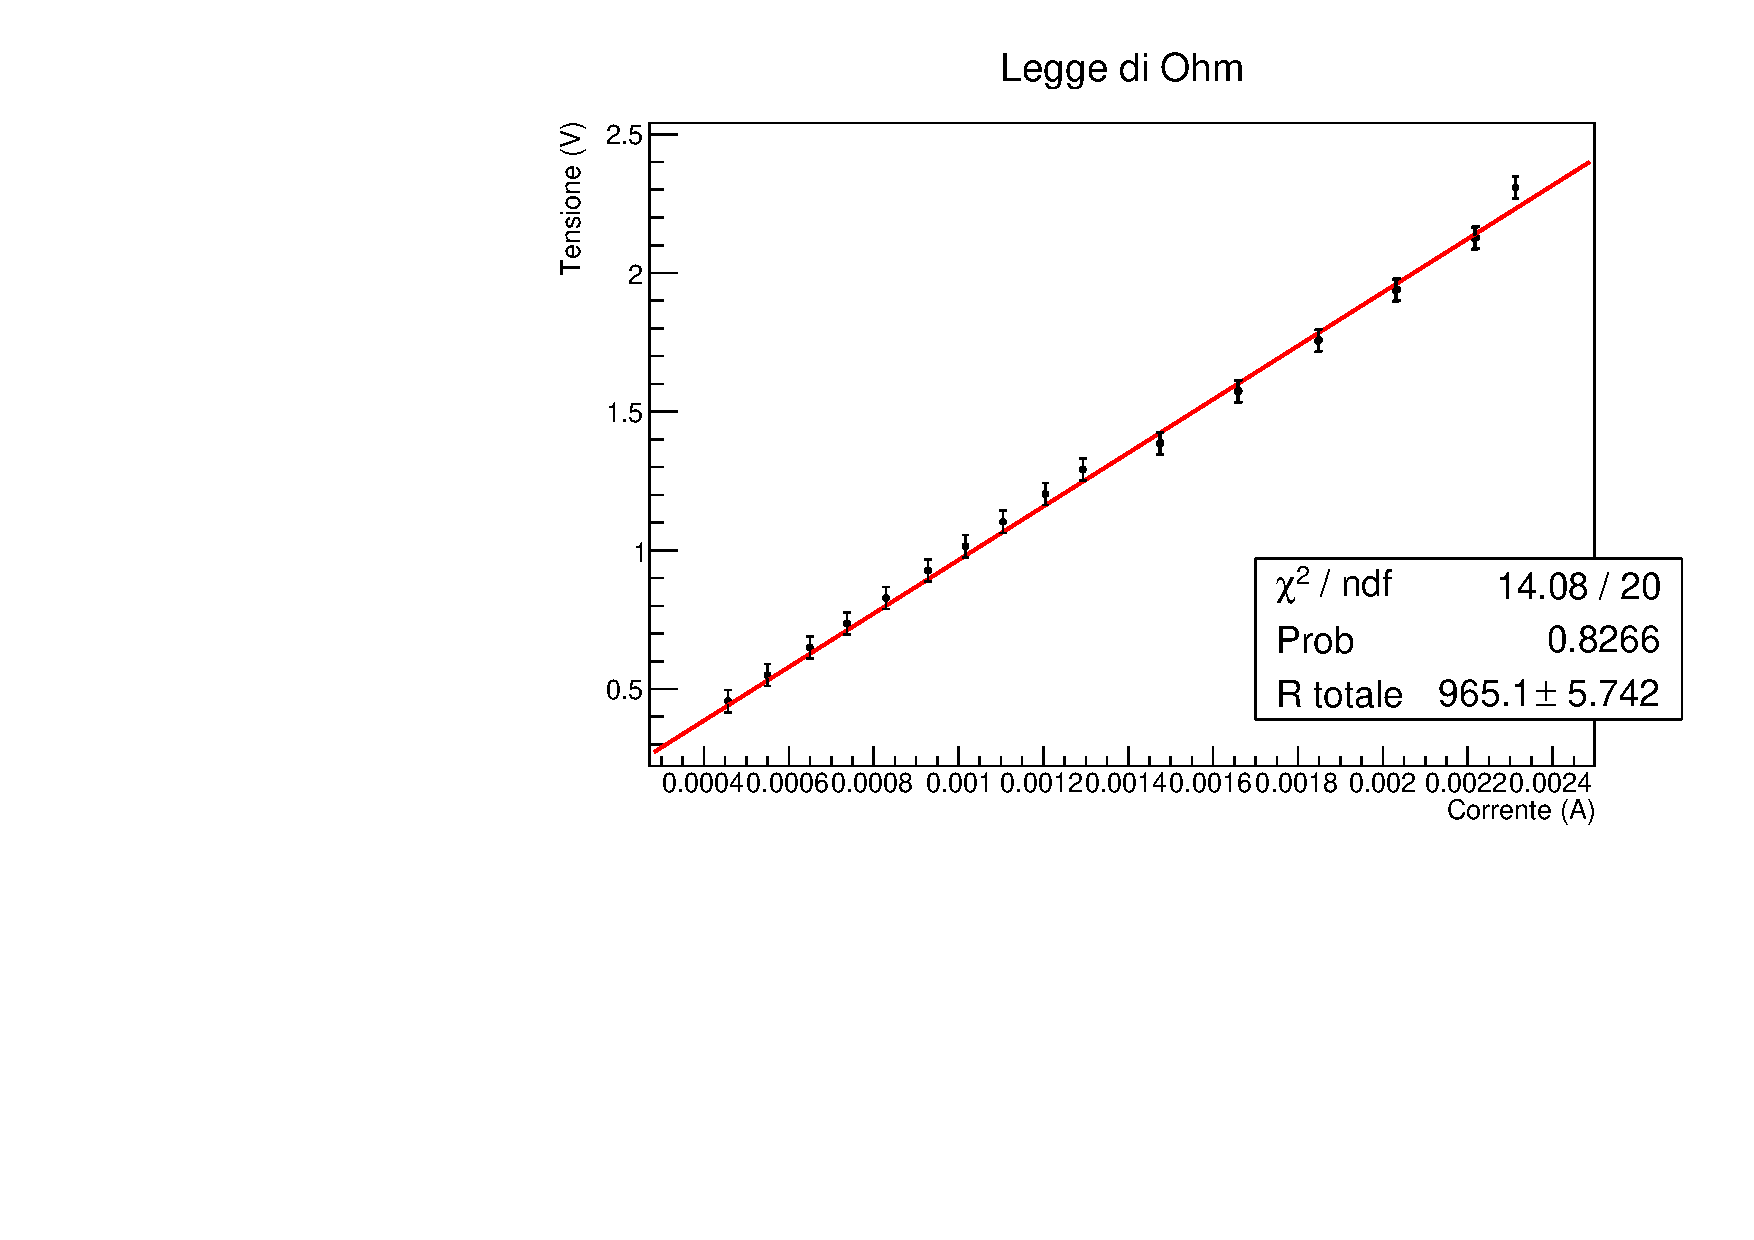
\includegraphics[scale=.45]{Immagini/fit3.pdf}
    \quad
    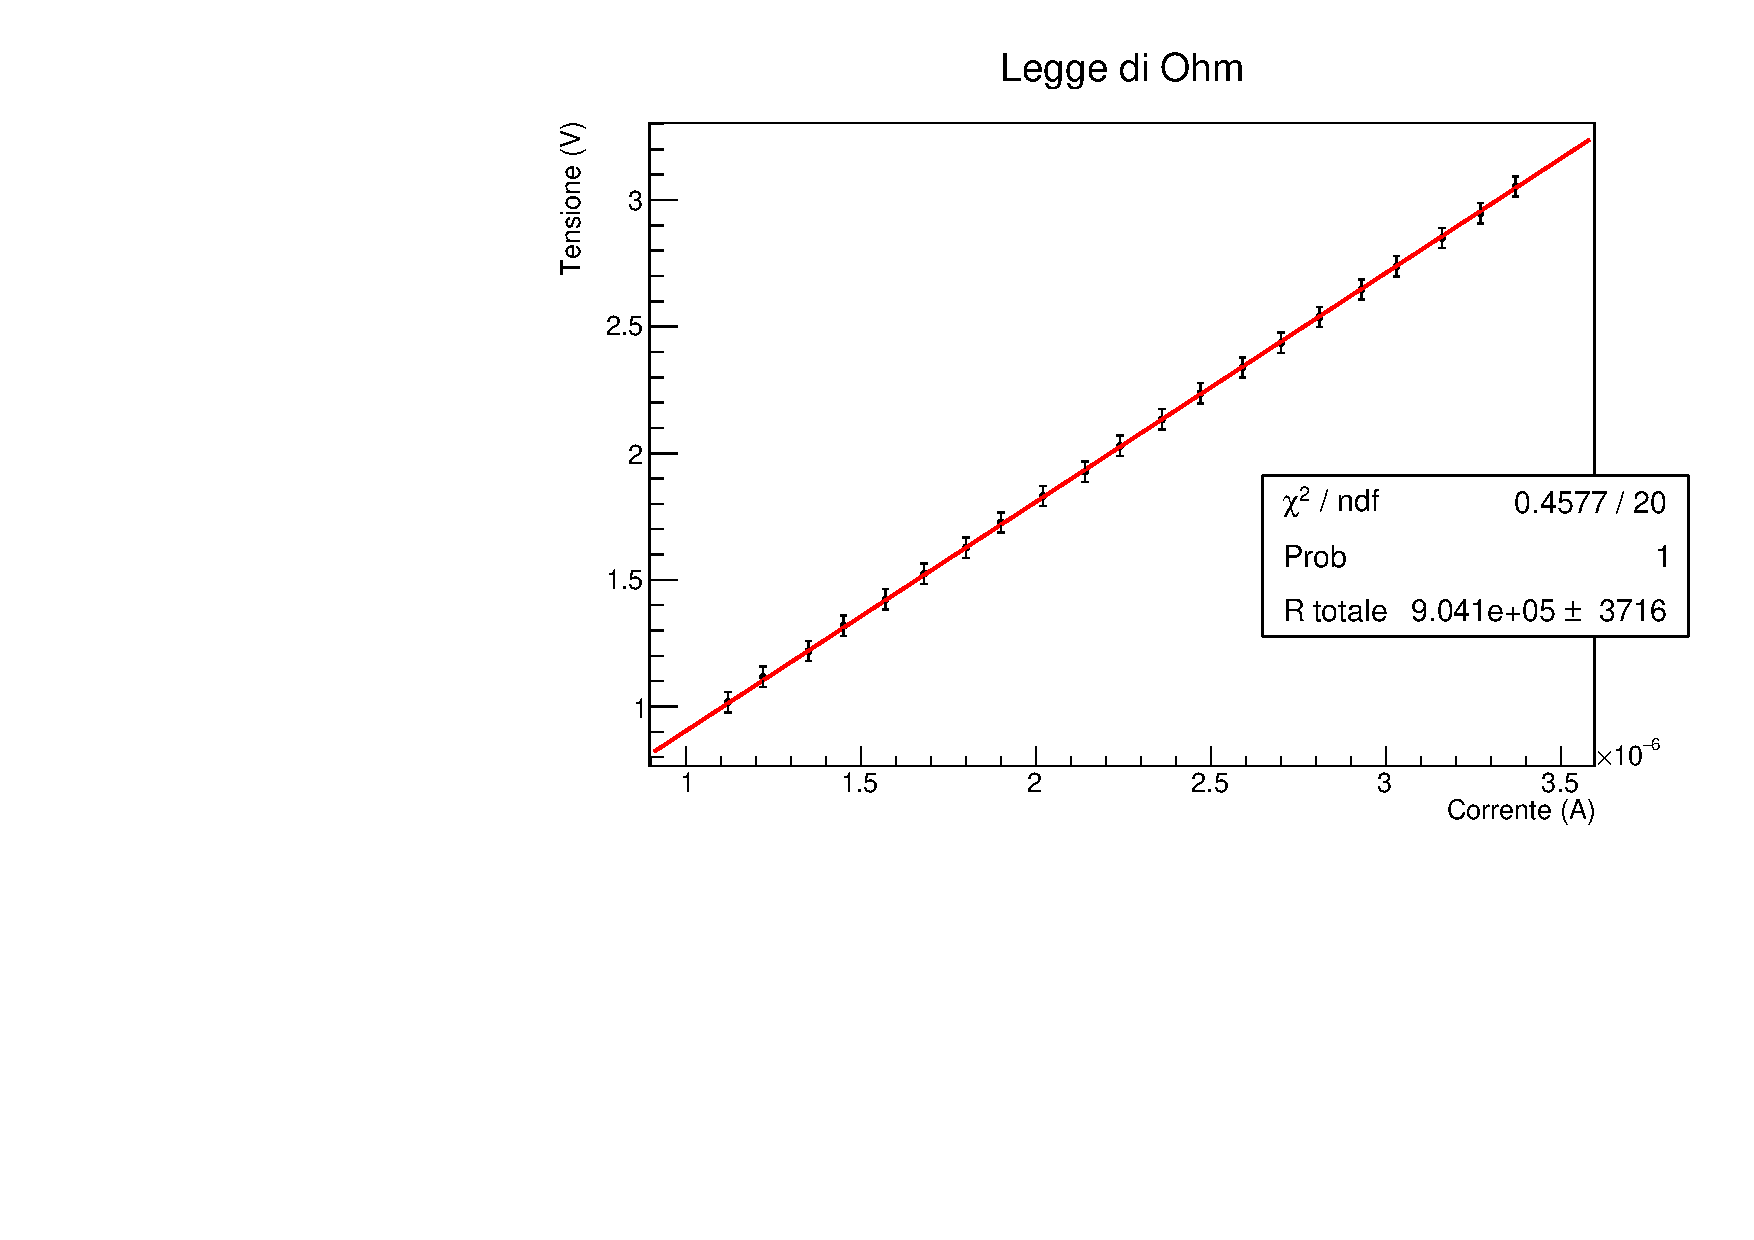
\includegraphics[scale=.45]{Immagini/fit4.pdf}
    \caption{Configurazione 1 in alto e configurazione 2 in basso}
\end{figure}


\subsection{Misura di resistenze composite}
Infine abbiamo disposto, prima in parallelo e poi in serie, due resistori (scelti con lo stesso ordine di grandezza della resistenza) e abbiamo verificato con essi la legge di Ohm. In questo caso abbiamo utilizzato solamente la configurazione 2, in quanto la misura che in precedenza avevamo ottenuto per $R_{V}$ poteva non essere corretta.

\begin{table}[H]
\parbox{.45\linewidth}{
    \centering
    \begin{tabular}{cc}
    \toprule
    $\Delta$ V (V)  & I (mA) \\
    \midrule
    0,503	&44,12\\
1,016	&89,15\\
1,519	&133,25\\
2,029	&177,94\\
2,538	&221,84\\
3,044	&265,8\\
3,551	&109,5\\
4,055	&352,8\\
    \bottomrule
    \end{tabular}
    \caption{Resistenze in parallelo; R_{tot}=5$\Omega$}
    \label{tab:my_label}
    }
    \quad
    \parbox{.45\linewidth}{
    \centering
    \begin{tabular}{cc}
    \toprule
    $\Delta$ V (V)  & I (mA) \\
    \midrule
    0,507	&23,916\\
1,016	&47,931\\
1,524	&71,92\\
2,029	&95,73\\
2,539	&119,76\\
3,048	&114,7\\
3,551	&167,36\\
4,065	&191,45\\
    \bottomrule
    \end{tabular}
    \caption{Resistenze in serie; R_{tot}=20$\Omega$}
    \label{tab:my_label}
    }
\end{table}
\noindent
I fit e i relativi risultati sono riportati nella Figura \ref{fit 56}.
\begin{figure}[h!]
    \centering
    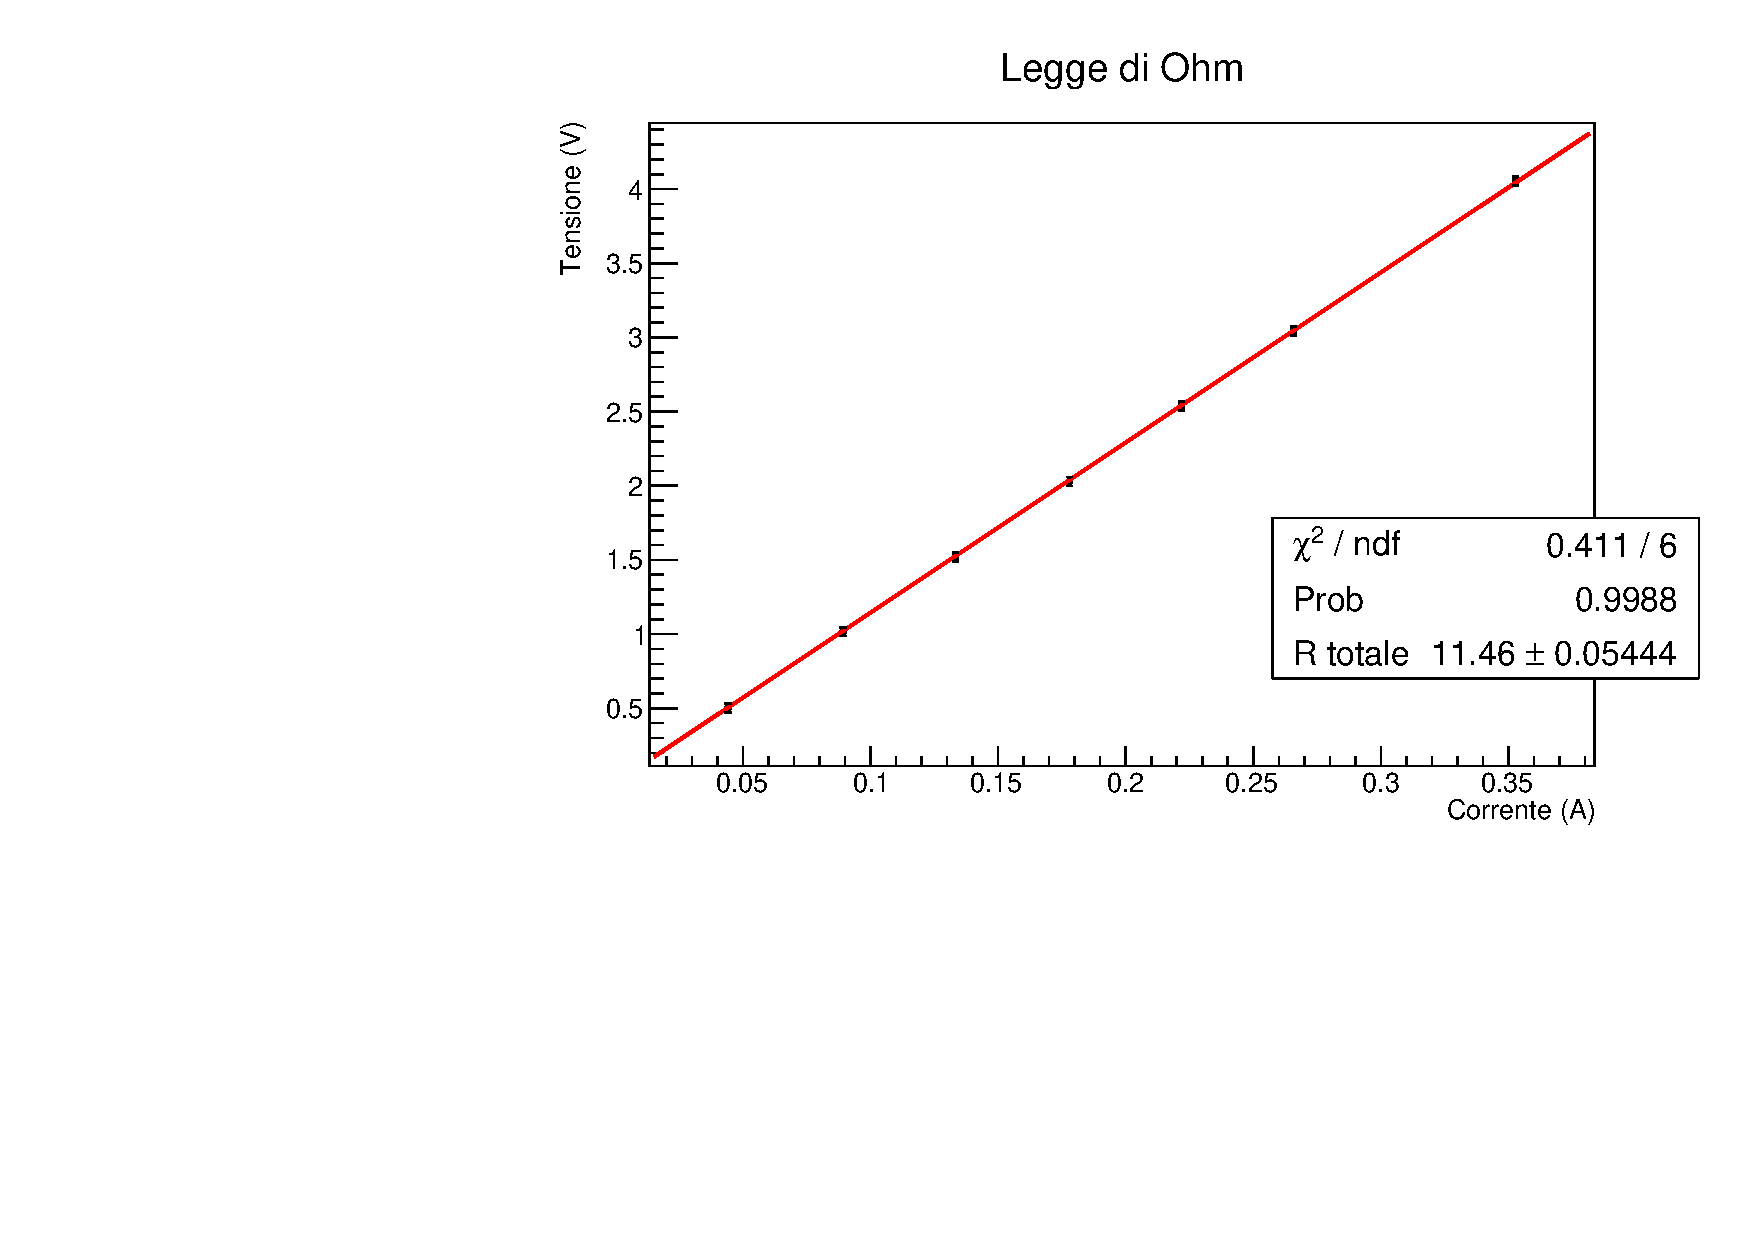
\includegraphics[scale=.4]{Immagini/fit5.pdf}
    \\
    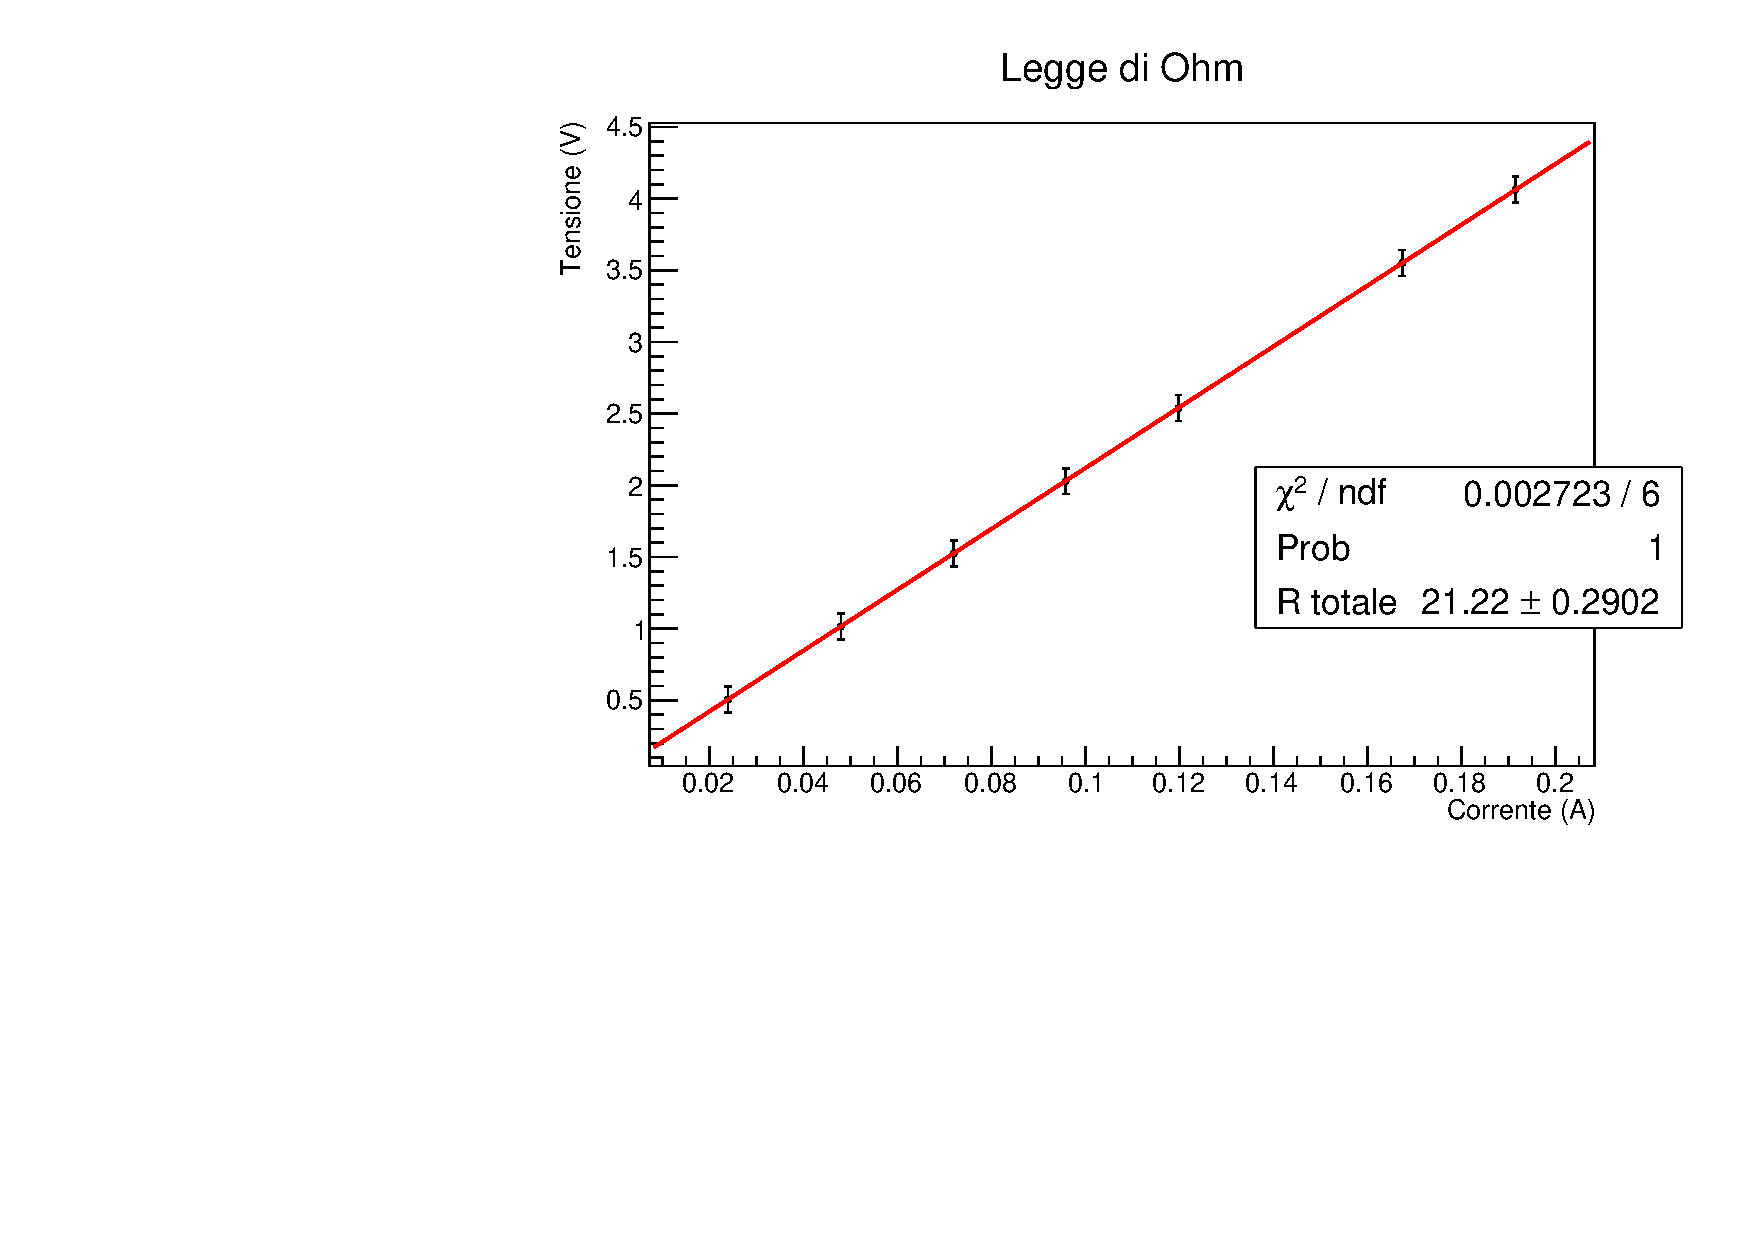
\includegraphics[scale=.4]{Immagini/fit6.pdf}
    \caption{}
    \label{fit 56}
\end{figure}